\documentclass{tudelftposter}
\usepackage{graphicx}
\usepackage{subfigure}
\title{TI2716-B License plate recognition, final poster}

\addauthornote{tu}{Group 2, Delft University of Technology}

\addauthor[tu]{Yinghao Dai}
\addauthor[tu]{Yanna van der Vlugt}

\addfootimage(c:right column.center)[Delft Institute of Applied Mathematics]{tudelft}

\begin{document}
\maketitle
\section{Introduction}
We are working on a license plate recogniser, which can, as the name already suggests, recognise license plates on cars under certain conditions. In the following, we will take you through the steps we have taken in order to correctly recognise a plate. 

\section{License plate detection and standardization}
The process of detecting a license plate in a frame is illustrated in figure \ref{1}. The frame (\ref{a}) is first thresholded to the colours of a license plate (\ref{b}). The recognised object is cropped out (\ref{c}) and the brightness and contrast are standardised using the function \texttt{imadjust} (\ref{d}). We then apply much stricter thresholds in order to separate the background from the letters. If necessary, the plate is rotated and remaining edges are cropped out. This leaves us with the characters in (\ref{e}). The largest six of these (so as to ignore any dirt, hyphens or other speckles on the plate) are individually cropped out fed through our character recognition function. If a large space between the current and a previous character is identified, a hyphen is put in this place. 

\begin{figure}[h]
	\centering
	\subfigure[Original image]{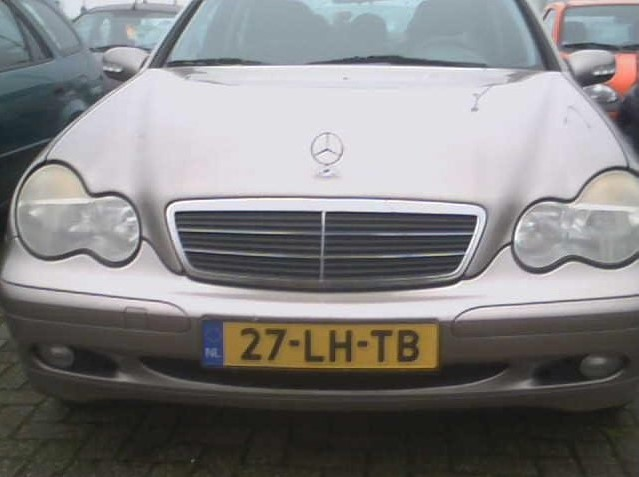
\includegraphics[width=500pt]{proces1.jpeg}\label{a}}
	\subfigure[Thresholding]{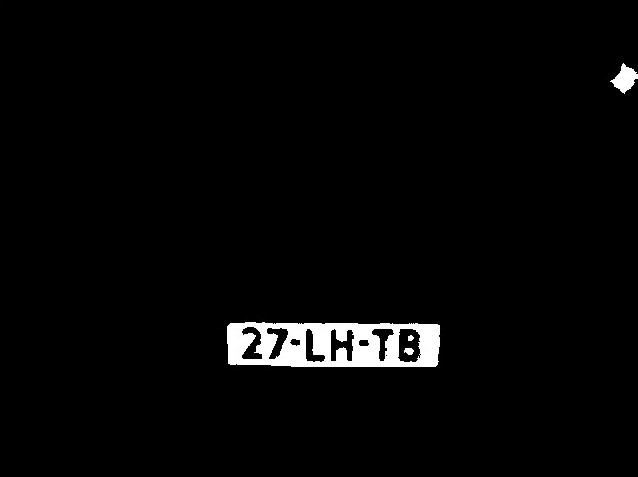
\includegraphics[width=500pt]{proces4.jpeg}\label{b}}
	\subfigure[Cropping]{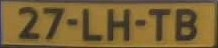
\includegraphics[width=300pt]{proces3.jpeg}\label{c}}
	\subfigure[Brightness/contrast]{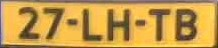
\includegraphics[width=300pt]{proces2.jpeg}\label{d}}
	\subfigure[Stricter thresholding]{
\includegraphics[width=300pt]{proces5.jpeg}\label{e}}
	\caption{Process of detecting and standardising a license plate.}
	\label{1}
\end{figure}

\section{Character recognition and format checking}
The character recognition function compares the individual characters with the possible characters in license plate font. If there are two possible characters that differ very little from the detected character, both are checked again with a heavier weighting for their differences. The resulting plate string is then fed through the format checker. In our example, the recognition function outputs `Z7-LH-T8', which is obviously not correct. Luckily, there are limited formats in which license plates appear, so we can use a format checker to find out that the plate should be `27-LH-TB'. If there is no suitable replacement so that the format is correct, the function outputs nothing, since this would definitely result in a false positive. 

\section{Graphical User Interface}
For an application like ours, a graphical user interface (GUI)
cannot be missing. A screenshot of the GUI is given in figure
\ref{gui}.

\begin{figure}[h]
	\centering
	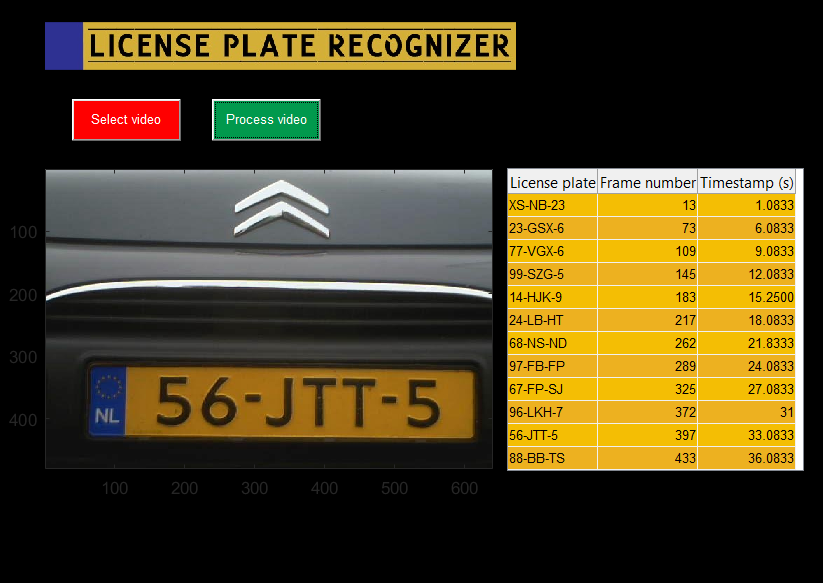
\includegraphics[width=800pt]{gui2.png}
	\caption{Graphical User Interface of our license plate recognizer.}
	\label{gui}
\end{figure}

\section{Improvements}
The most important change this week, that increased our score by 20\%, was post-processing the data. Previously, the GUI would output every located and format-checked license plate, which resulted in a lot of false positives. By only outputting the license plate that was located most often, our system no longer output plates where there was a mistake in the recognition. Calculating the Levenshtein distance between detected plates told us when a new plate was detected, due to our assumption that the distance between two different plates would be at least 3. 

\section{Score}
All these theoretical ideas are nice, but since the results make or break the quality of our recogniser, they are at least as important. The score after running the file \texttt{TrainingVideo.avi}, can be found in figure \ref{score}. 

\begin{figure}[h]
	\centering
	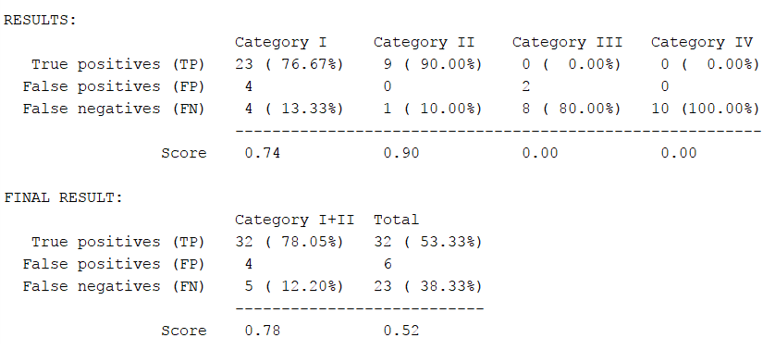
\includegraphics[width=800pt]{score.png}
	\caption{Results after running \texttt{TrainingVideo.avi}.}
	\label{score}
\end{figure}


\end{document}

%\experimentalblockright{%
%  SPAM:
%  Nulla malesuada porttitor diam. Donec felis erat, congue non, volutpat at,
%  tincidunt tristique, libero.}
